% !Mode:: "TeX:UTF-8"
\chapter{分支预测器介绍}


本章首先介绍香山处理器第二版分支预测的整体架构,各个预测器在流水级中的先后关系和联系。其次针对每个预测器都介绍了它们的预测原理和功能。

\section{分支预测整体结构}

香山第二版分支预测架构采用的是4级流水设计,架构图如图2.1所示。在4个流水级中,S0主要负责收集S1、S2、S3流水级的预测结果,以及取指单元和流水线后端发挥的分支误预测信息,从中选择出下一周期需要进行预测的pc,然后将该pc对应的读请求发给各个预测器,不同的预测器得出预测结果的时间需要1到2周期不等。

由于更加准确的预测器得出预测结果需要的时间更久,为了能够让分支预测流水线无气泡的流水,因此首先需要一个0-bubble的预测器,也就是负责在S1做出预测的Micro BTB,它每周期都能够针对上一个周期的pc给出预测结果,及时的给出下一周期需要预测的pc,这样就能够让流水线无气泡的工作。之后S2是由FTB、TAGE和RAS联合做出的预测结果,由于S2的算法更复杂,能够覆盖更多的情况,因此我们认为它的预测准确率高于S1。当出现S2的预测跳转方向和跳转目标地址和S1预测的结果不相同时,我们会以S2的预测结果为准,这意味着之前S1预测的结果需要修正,需要清空S2之前的流水线,从S2预测的下一周期目标地址开始重新预测,这时分支预测流水线就会产生1拍的气泡。同样的,在S3会使用SC和ITTAGE再进行一次预测, 我们认为这次的预测是最准确的,也就是说S2的预测结果和S3预测结果不同时以S3的结果为准。当出现S2和S3预测结果不同时,也需要刷新分支预测流水线重新取指,这会带来2周期的气泡。

\begin{figure}[htb]
	\centering
	\setlength\tabcolsep{3pt}  % 同一行中的图片间隔
	\vspace{5pt} % 图片上部的空白,如果太小的话,图片顶部会与正文内容十分接近
	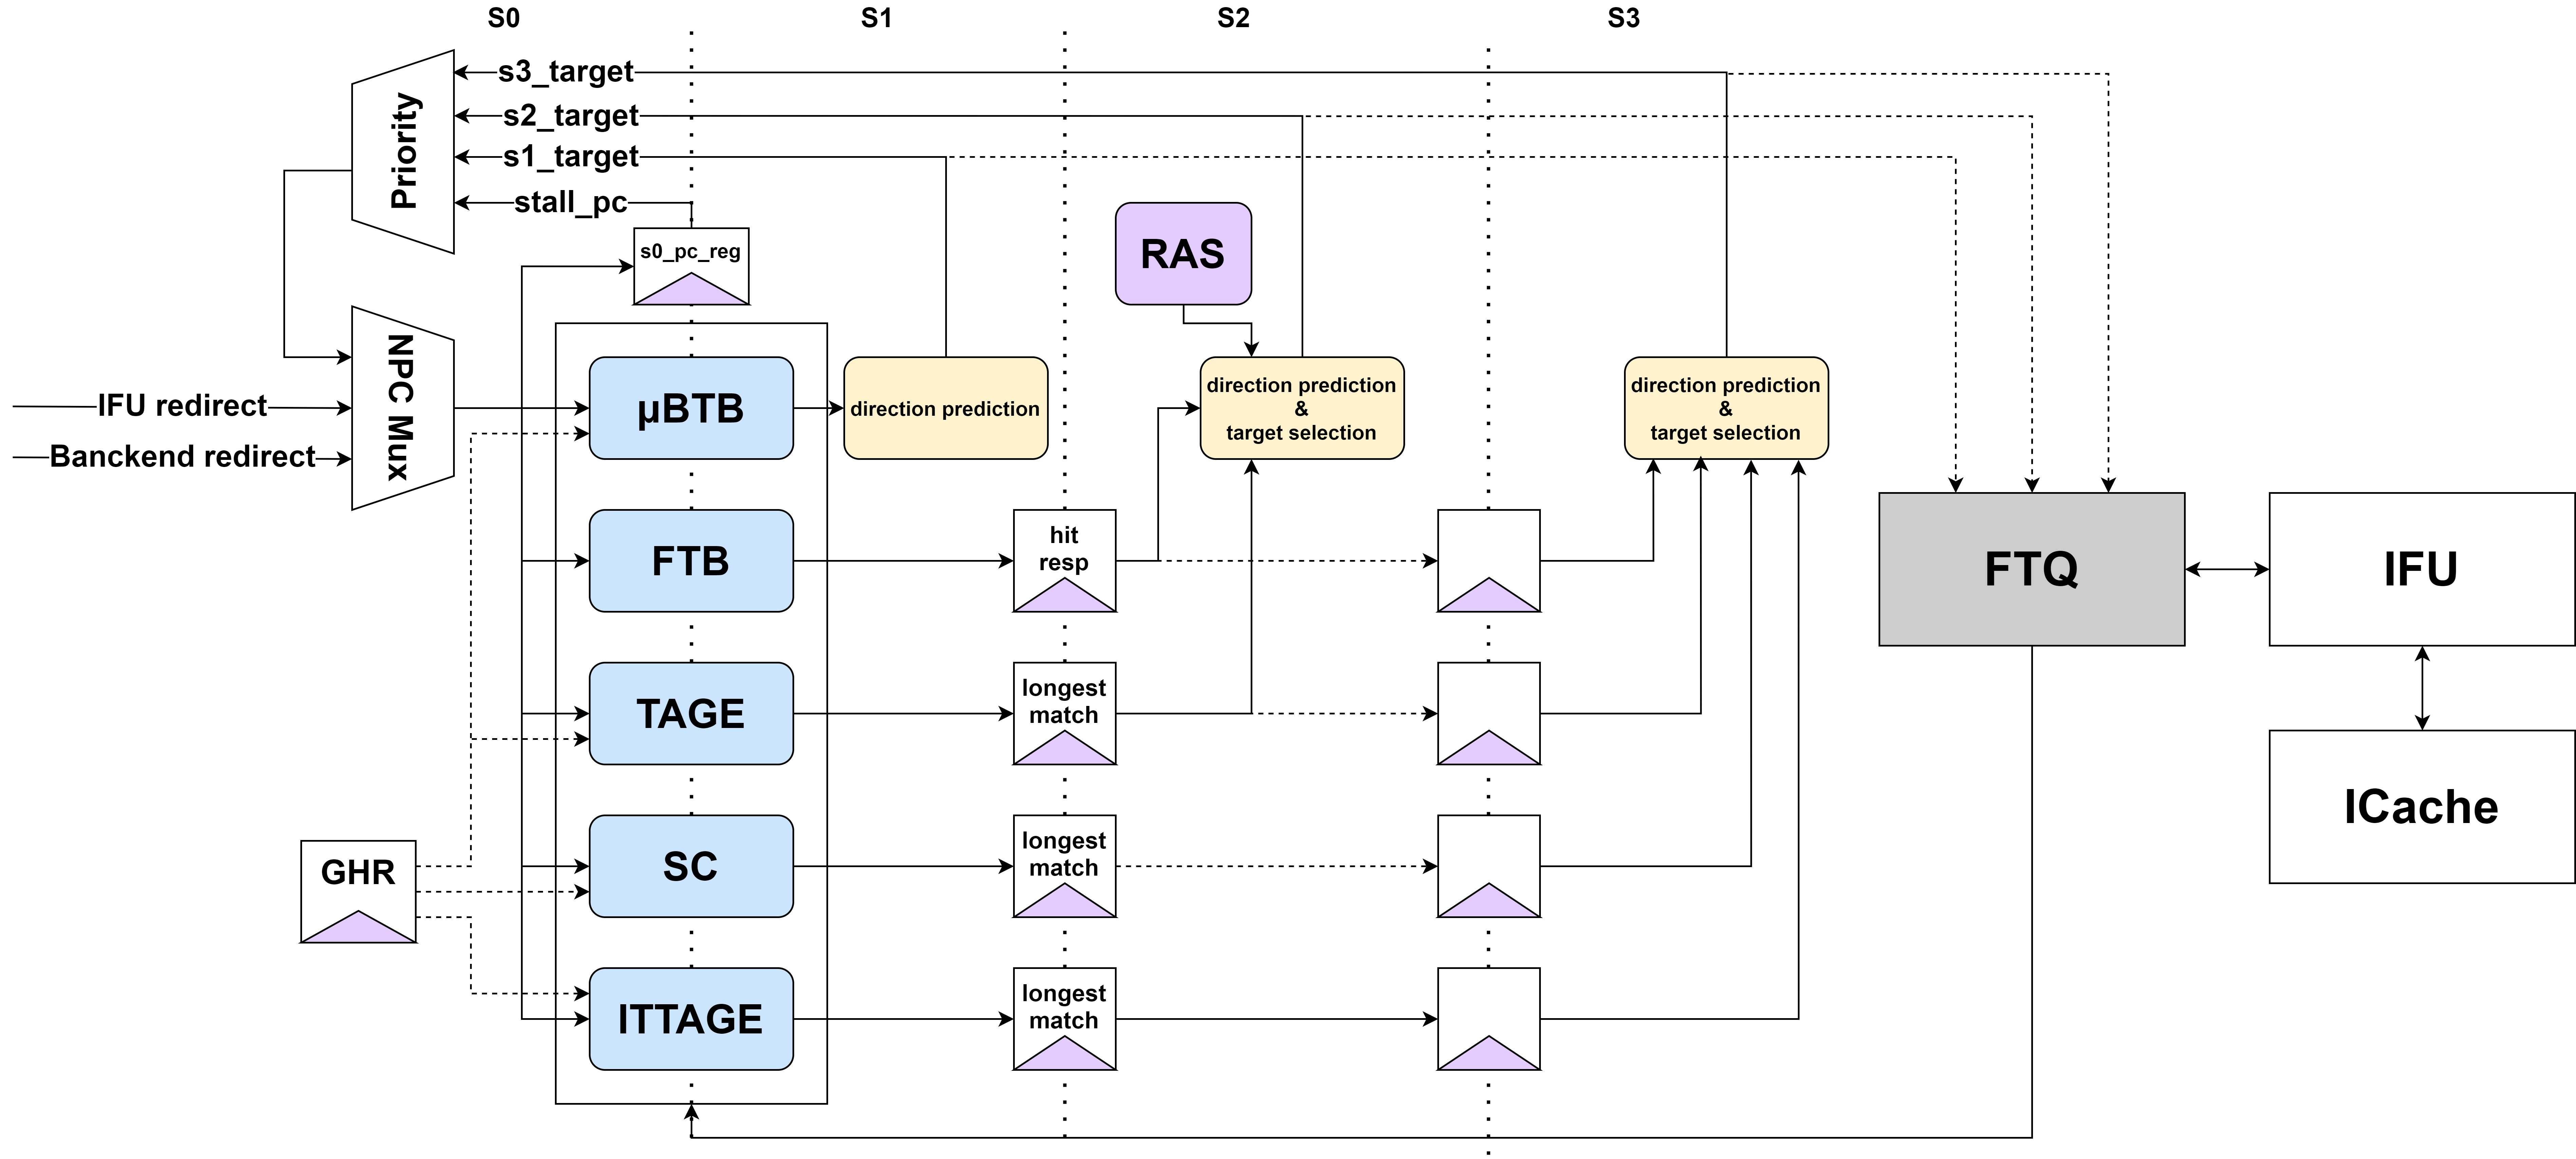
\includegraphics[width=1\textwidth]{BPU-FTQ-IFU.jpg}
	\caption{香山处理器第二版分支预测架构图}
	\label{fig:figure1}
\end{figure}

\section{FTB设计介绍}

由于分支预测执行在取指之前,因此我们无法通过对指令码进行预译码来识别一条指令是否是分支指令,也无法知道一条分支指令的跳转目标地址,因此我们需要在分支指令执行完毕时将它们保存在一个Buffer中,通过它们的pc进行索引,这样下次再遇到同一条分支指令时,我们就可以通过查找这个Buffer来获得它的相关信息,从而得知它的指令类型和跳转目标地址。这就是FTB (Fetch Target Buffer) 的主要功能。它负责在预测时指出哪些指令是分支指令,以及它们对应的跳转目标地址。

\section{Micro BTB设计介绍}

Micro BTB作为一个0-bubble的预测器,首先具有一个小型FTB的功能,它也能够保存分支指令的信息,但是由于它需要在很快的时间内做出一个初步的预测,因此它的逻辑必须简单,使用的硬件资源必须足够小,因为过于复杂的逻辑和过多的面积都会导致它无法按时给出预测结果。Micro BTB会使用pc和全局历史做索引,当Micro BTB命中,即发现当前pc对应的取指块已经被保存时,它会依据上一次索引到该项的分支的跳转方向,以此作为这次的预测结果。

\section{RAS设计介绍}

RAS (Return Address Stack) 是一个专门针对call和return指令优化的预测器。我们知道在程序执行某个函数时,首先会使用一条call指令跳转到函数的起始地址,然后函数的最后会有一条return指令,再将程序跳转回call指令之后的下一条指令继续执行。由于函数调用是递归的,因此可以使用一个栈结构来保存所有函数调用的返回地址。当检测到一条call指令时,将这条call指令之后的下一条指令存入RAS,然后当检测到一条return指令时,就将RAS栈顶保存的地址出栈,作为这条return指令的跳转目标地址。

\section{TAGE设计介绍}

TAGE (TAgged GEometric history length branhc predictor) 是在2004年第一件分支预测大赛上由André提出的一种预测器,之后不断地优化和改进,多次夺得了分支预测大赛的冠军,也是目前公开的分支预测性能最好的预测器。TAGE是一个使用全局历史索引的方向预测器,也就是说它只会用来预测分支是否跳转,而跳转目标地址需要由FTB、RAS或ITTAGE来提供。
TAGE由多张预测表组成,每张表通过不同长度的分支历史来索引,表中的每一项都是一个饱和计数器。每次预测时会同时查找所有的表,然后从中选择出历史长度最长且tag匹配的表,以它的饱和计数器值作为分支预测的结果。

\section{SC设计介绍}

SC (statistical corrector) 是TAGE预测器的一个组件,用来预测一部分TAGE不能准确预测的分支指令,即与全局历史没有太多相关性,但是跳转方向有明显的偏向值的分支。

\section{ITTAGE设计介绍}

ITTAGE (Indirect Target TAgged GEometric history length branhc predictor) 是一个专门针对间接跳转分支的预测器,其算法大部分与TAGE相同。不同之处在于TAGE中用于判断跳转方向的饱和计数器被替换成了一个跳转目标地址和一个置信度计数器

\section{本章小结}

本章主要详细介绍了本文提出的分支预测架构的流水线设计和工作流程,单独列出了多个预测器的功能和算法